\section{Priklijst}

    \vspace{-6em}

    \begin{center}
    \includegraphics[scale=.7]{priklijst1}
    \vspace{-6em}
    \includegraphics[scale=.7]{priklijst2}
    \end{center}


\section{Bedradingsschema}


    %\begin{figure}
    \begin{center}
    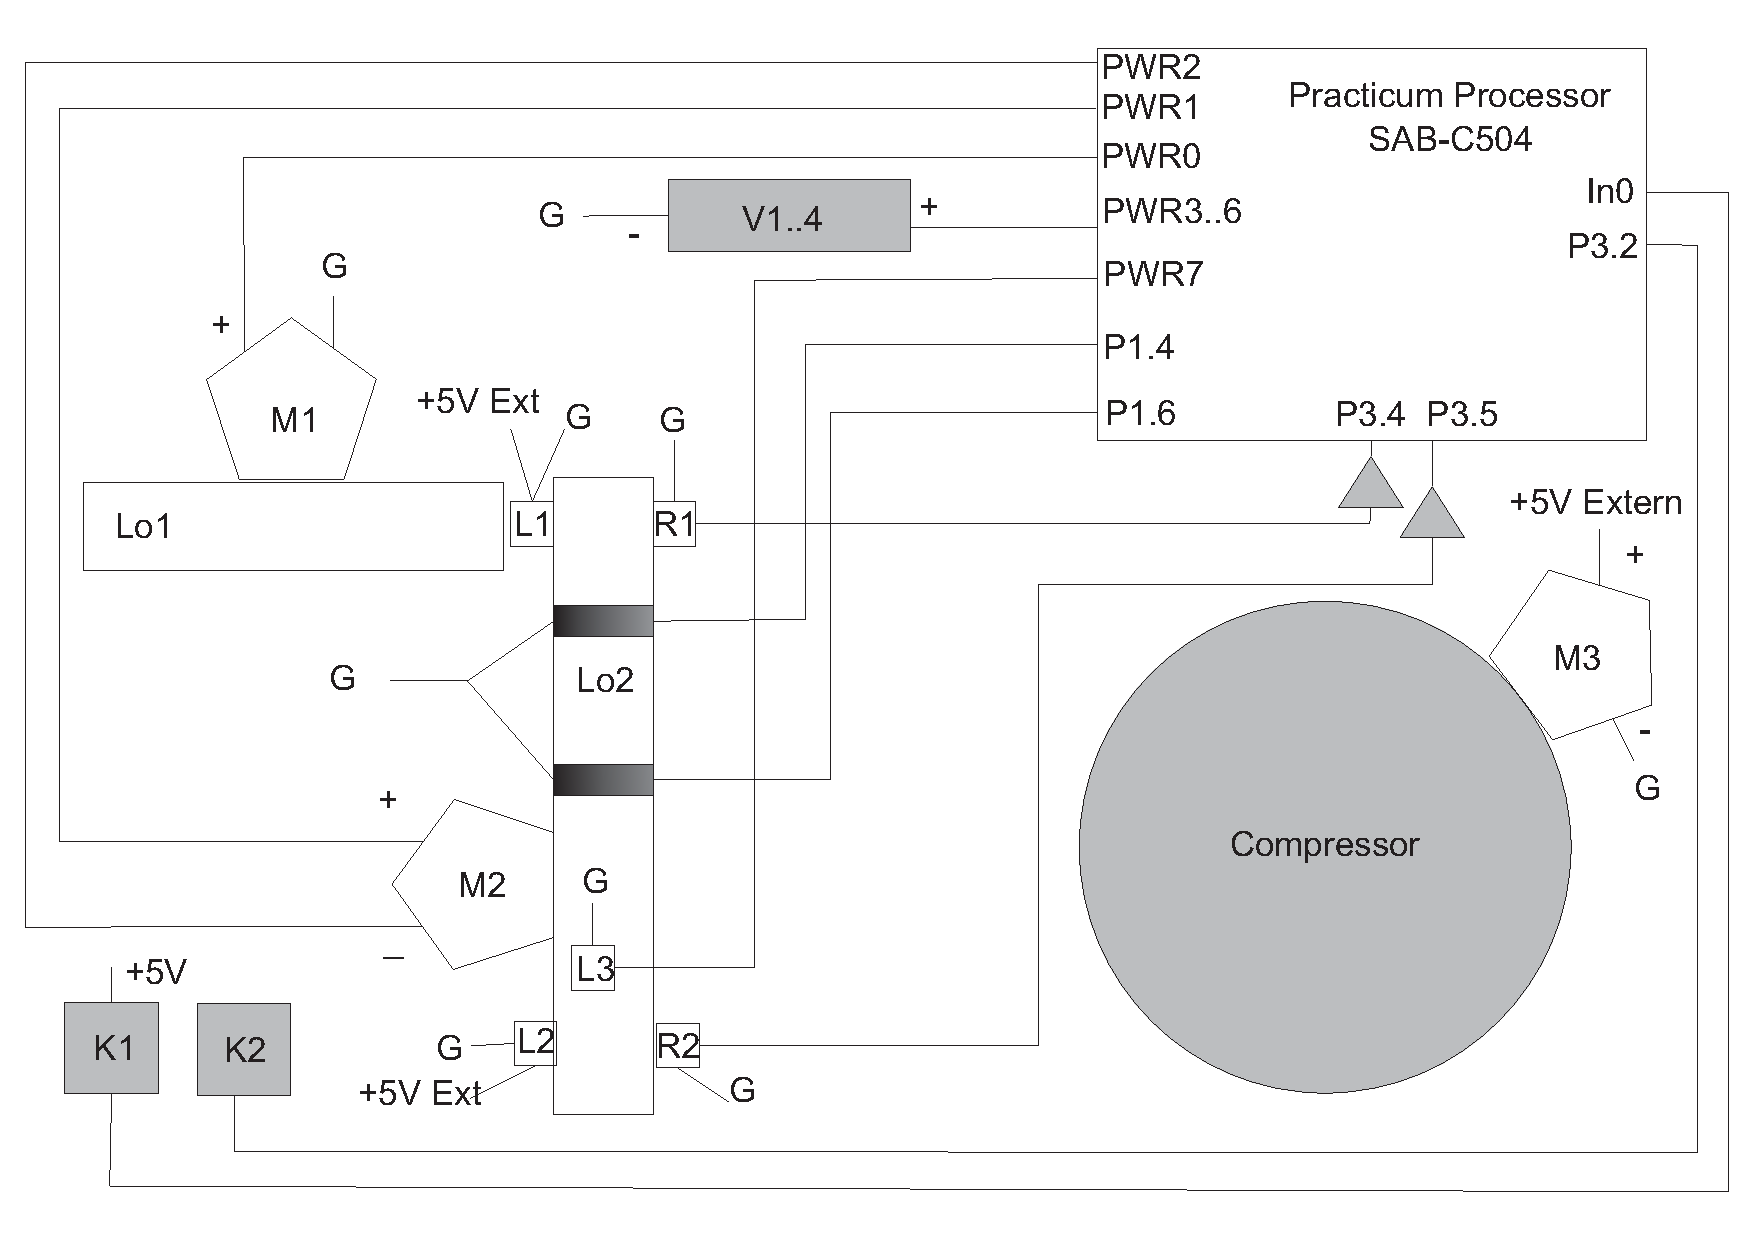
\includegraphics[scale=.5]{bedrading}
    \end{center}
    %\end{figure}

\section{Beluchtingsschema}


    %\begin{figure}
    \begin{center}
    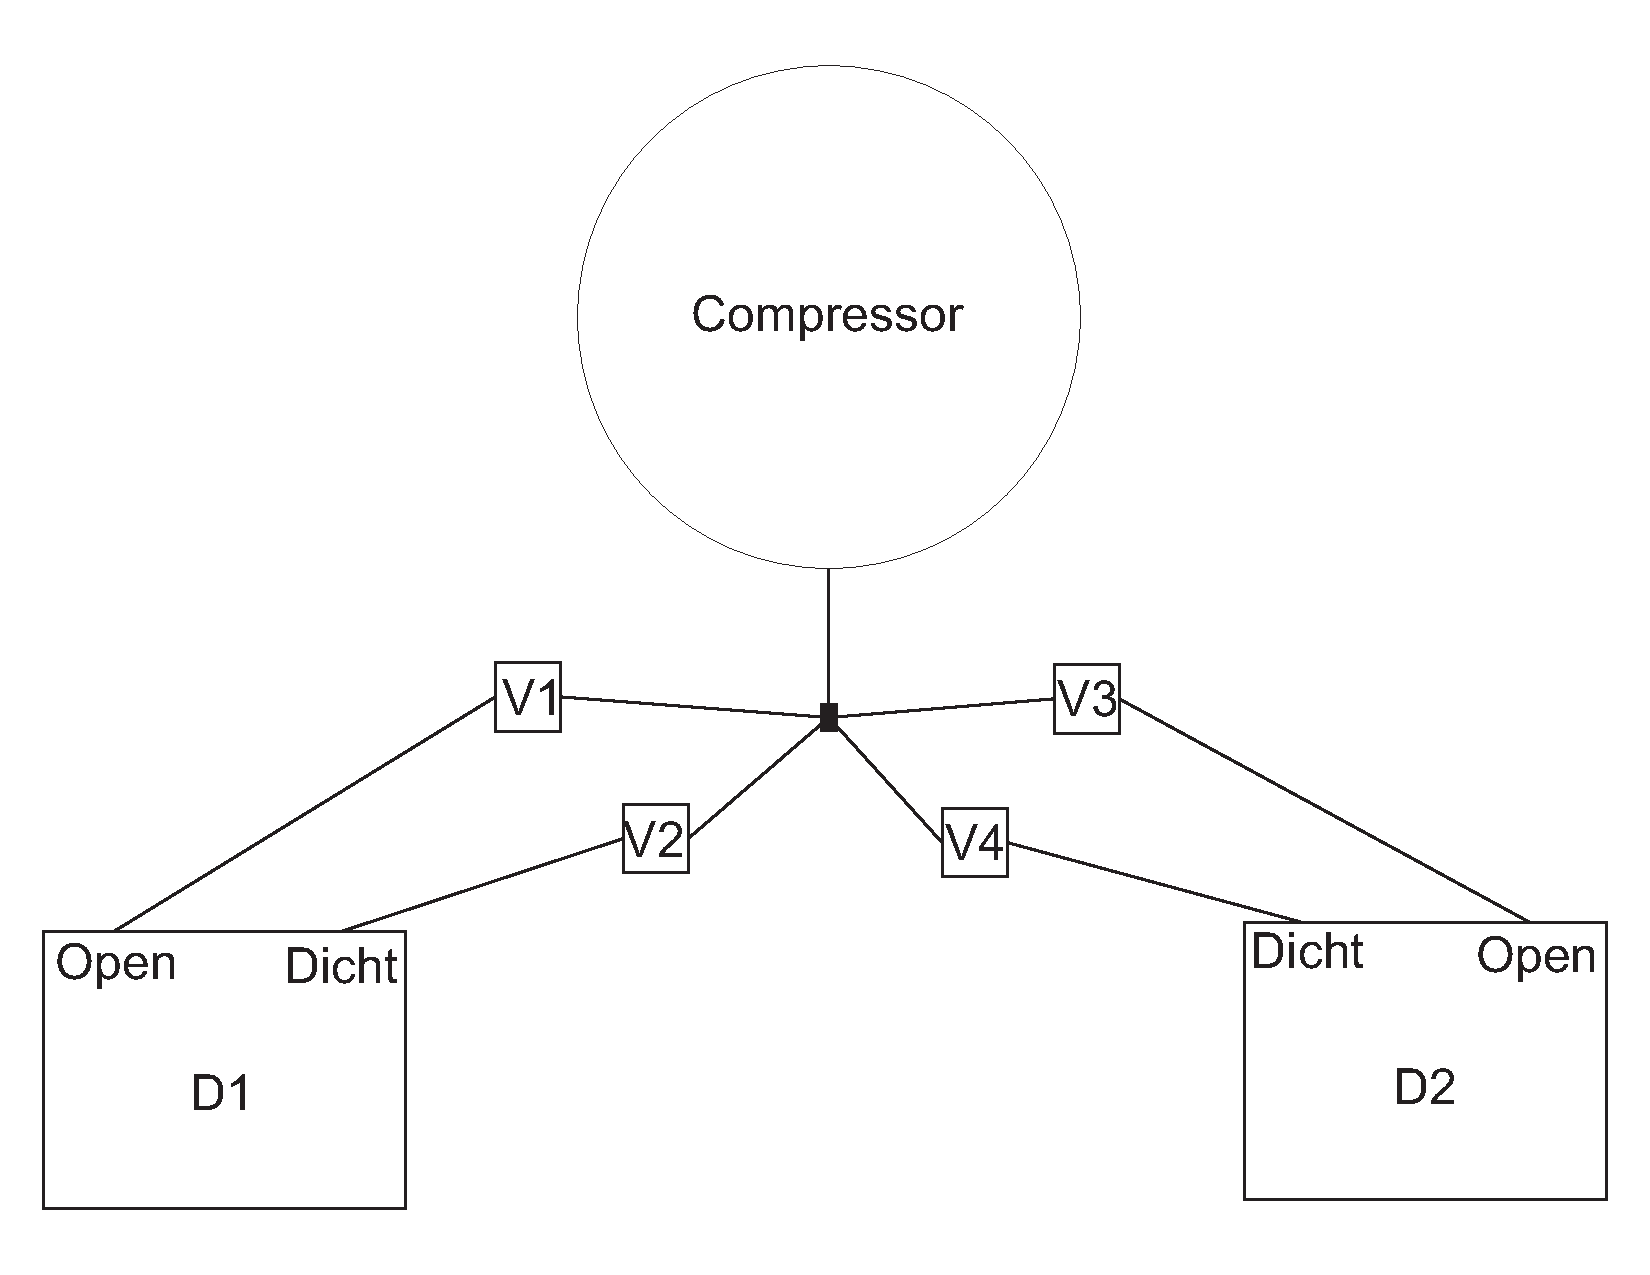
\includegraphics[scale=.5]{beluchting}
    \end{center}
    %\end{figure}

    We gebruiken \'{e}\'{e}n compressor waarop vier luchtkleppen zijn
    aangesloten. E\'{e}n luchtklep dient om deur 1 te openen,
    \'{e}\'{e}n om deur \'{e}\'{e}n te sluiten, er is er \'{e}\'{e}n om deur twee
    te openen, de laatste sluit deur twee. We hebben overwogen om
    \'{e}\'{e}n luchtklep te gebruiken om beide deuren te sluiten,
    omdat toch nooit beide deuren gelijk open mogen zijn. We hadden
    toen echter ons beluchtingsschema al ingeleverd en hebben het
    dus maar bij het originele ontwerp gelaten.
